\documentclass{article}

\usepackage{amsmath}
\usepackage{graphicx}
\usepackage{hyperref}

\title{CSCI 5942: AI Engineering Assignment 1}
\author{Bill Hsu}
\date{September 3, 2026}

\begin{document}

\maketitle

\section{Deliverables:}

\begin{figure}[ht]
    \centering
    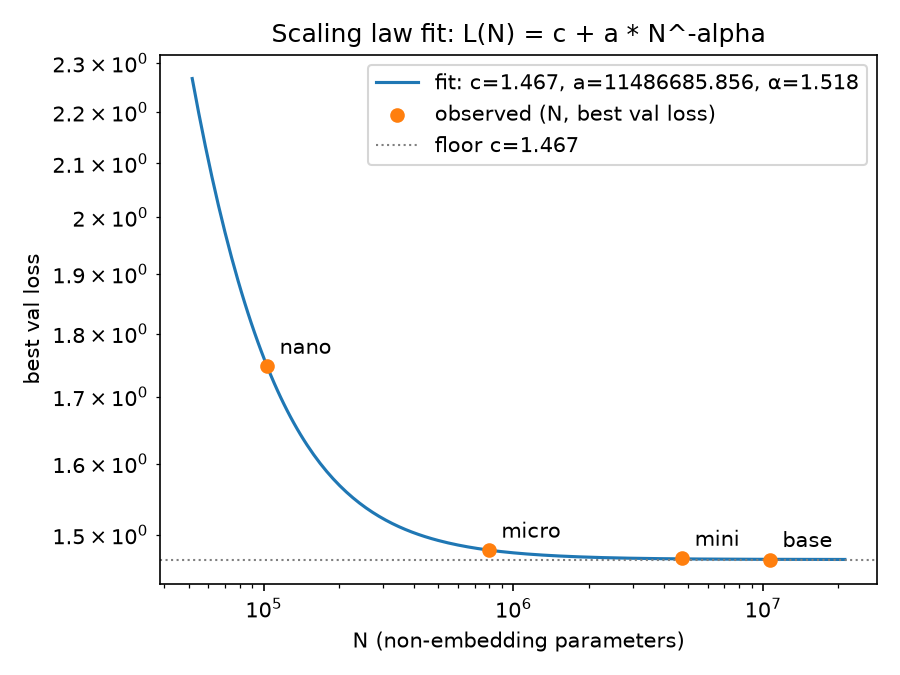
\includegraphics[width=1.0\textwidth]{scaling_law.png}
    \label{fig:scaling_law}
\end{figure}

\section{URL of model.py}

\url{https://drive.google.com/file/d/1Orbrv8ilIs3z-0m4B1rHi_u9YCHw7wOM/view?usp=sharing}

\section{Answer to the questions in Part 3}

\begin{enumerate}
    \item The token/N of base is about 7.69, way more lower than the token/N of 20, which Chinchilla found to be optimal. 
    In other words, the base model has more parameters than it's 82M training tokens can support.
    This puts it on the side that needs more training tokens, not more parameters.
    \item From the plotting, C is about 1.4668. This floor reflects the fact that entropy inherent in the task,
    which no model can remove nomather how larger or well-trained.
    \item The fit result shows that adding parameters at a fixed token budget (mini to base) produced almost no improvement in loss. 
    Based on the fit, if we could double the training data rather than parameters, we have higher potential to reduce the loss.
\end{enumerate}


\end{document}